\documentclass{sigchi}

% Use this command to override the default ACM copyright statement (e.g. for preprints). 
% Consult the conference website for the camera-ready copyright statement.


%% EXAMPLE BEGIN -- HOW TO OVERRIDE THE DEFAULT COPYRIGHT STRIP -- (July 22, 2013 - Paul Baumann)
% \toappear{Permission to make digital or hard copies of all or part of this work for personal or classroom use is  granted without fee provided that copies are not made or distributed for profit or commercial advantage and that copies bear this notice and the full citation on the first page. Copyrights for components of this work owned by others than ACM must be honored. Abstracting with credit is permitted. To copy otherwise, or republish, to post on servers or to redistribute to lists, requires prior specific permission and/or a fee. Request permissions from permissions@acm.org. \\
% {\emph{CHI'14}}, April 26--May 1, 2014, Toronto, Canada. \\
% Copyright \copyright~2014 ACM ISBN/14/04...\$15.00. \\
% DOI string from ACM form confirmation}
%% EXAMPLE END -- HOW TO OVERRIDE THE DEFAULT COPYRIGHT STRIP -- (July 22, 2013 - Paul Baumann)


% Arabic page numbers for submission. 
% Remove this line to eliminate page numbers for the camera ready copy
% \pagenumbering{arabic}


% Load basic packages
\usepackage{balance}  % to better equalize the last page
\usepackage{graphics} % for EPS, load graphicx instead
\usepackage{times}    % comment if you want LaTeX's default font
\usepackage{url}      % llt: nicely formatted URLs
\usepackage{siunitx}
\usepackage{cite}
\usepackage{dblfloatfix}

% llt: Define a global style for URLs, rather that the default one
\makeatletter
\def\url@leostyle{%
  \@ifundefined{selectfont}{\def\UrlFont{\sf}}{\def\UrlFont{\small\bf\ttfamily}}}
\makeatother
\urlstyle{leo}


% To make various LaTeX processors do the right thing with page size.
\def\pprw{8.5in}
\def\pprh{11in}
\special{papersize=\pprw,\pprh}
\setlength{\paperwidth}{\pprw}
\setlength{\paperheight}{\pprh}
\setlength{\pdfpagewidth}{\pprw}
\setlength{\pdfpageheight}{\pprh}

% Make sure hyperref comes last of your loaded packages, 
% to give it a fighting chance of not being over-written, 
% since its job is to redefine many LaTeX commands.
\usepackage[pdftex]{hyperref}
\hypersetup{
pdftitle={Skintillates: Towards Epidermal Interactions},
pdfauthor={LaTeX},
pdfkeywords={SIGCHI, proceedings, archival format},
bookmarksnumbered,
pdfstartview={FitH},
colorlinks,
citecolor=black,
filecolor=black,
linkcolor=black,
urlcolor=black,
breaklinks=true,
}

% create a shortcut to typeset table headings
\newcommand\tabhead[1]{\small\textbf{#1}}
\newcommand{\ignore}[1]{}


% End of preamble. Here it comes the document.
\begin{document}

\title{Skintillates: Towards Epidermal Interactions}

\numberofauthors{3}
\author{
  \alignauthor 1st Author Name\\
    \affaddr{Affiliation}\\
    \affaddr{Address}\\
    \email{e-mail address}\\
    \affaddr{Optional phone number}
  \alignauthor 2nd Author Name\\
    \affaddr{Affiliation}\\
    \affaddr{Address}\\
    \email{e-mail address}\\
    \affaddr{Optional phone number}    
  \alignauthor 3rd Author Name\\
    \affaddr{Affiliation}\\
    \affaddr{Address}\\
    \email{e-mail address}\\
    \affaddr{Optional phone number}
}

\maketitle

\begin{abstract}
Beyond phones, watches, and activity tracking devices, a new ecosystem of functional and fashionable wearable technologies can easily, safely, and economically be designed, prototyped, and integrated directly on the skin. Skintillates is a wearable technology that mimics tattoo - the oldest and most commonly used on-skin display in human culture. We demonstrate that by fabricating sensors and thin electronics on temporary tattoo paper, a wide array of displays and sensors can be created. Just like the non-functionalized temporary tattoo often worn by children to adults alike, the Skintillates devices flex naturally with the user's skin. Our simple fabrication technique also enables users to freely design and print with full range of colors to customize for their specific applications. In addition to demonstrating the technical capability of Skintillates in the application examples, we also briefly explore how Skintillates, an electronic augmented tattoo, can serve as a platform for the combination of public and private body art and displayed data. (needs trim) 
\end{abstract}

\keywords{
  Fabrications; wearable  \newline
}

\category{H.5.m.}{Information Interfaces and Presentation (e.g. HCI)}{Miscellaneous}

\section{Introduction}
\begin{figure}[!h]
\centering
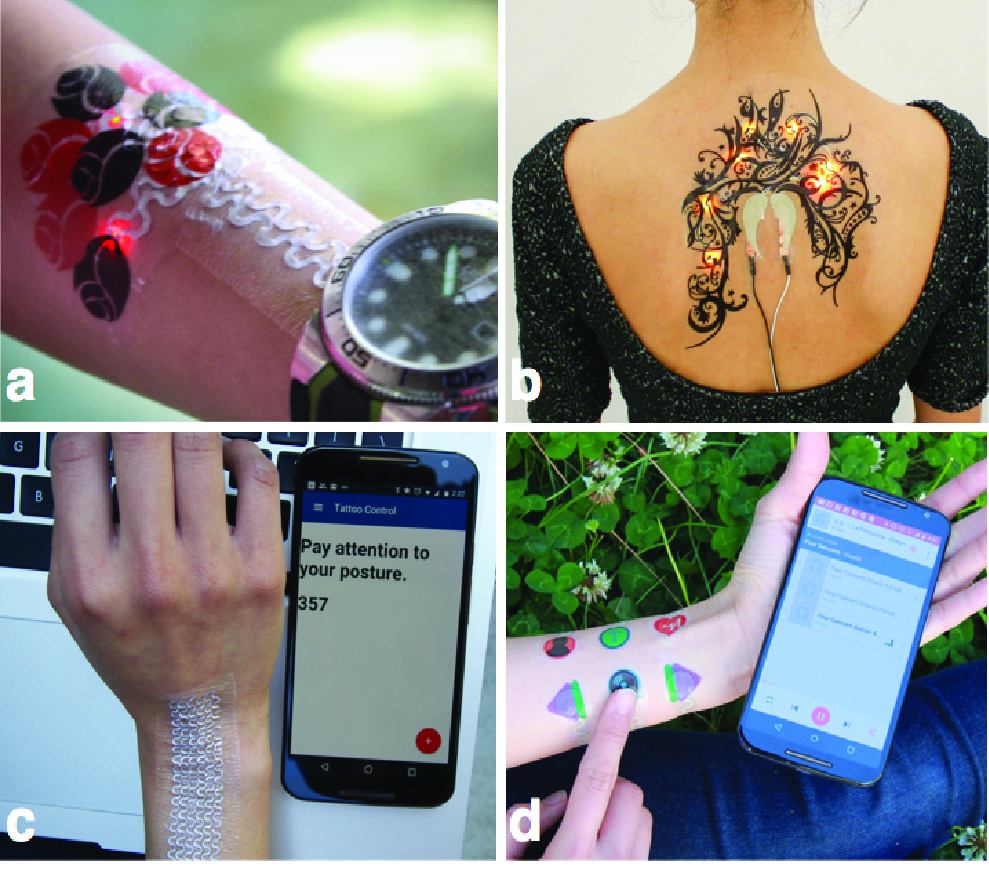
\includegraphics[width=1\columnwidth]{figures/Figure1}
\caption{Skintillates is a tattoo interactive platform that can be fabricated with an accessible process.}
\label{fig:figure1}
\end{figure}
Everyday, we interact with the world through our skin. The human skin senses important events that happen closest to us, and serves as an expressive medium when adorned with tattoo art. In this paper, we present Skintillates, a class of temporary tattoo epidermal wearable interactive devices. Skintillate devices presented in this paper include electronic tattoo as passive and active on-skin display, capacitive sensors for mobile devices electronic instrument control and strain gauge for posture detection. Similar to traditional tattoo, Skintillates can be customized to be a variety of different sizes and colors to fit the user’s intended functions. Moreover, we demonstrate an accessible fabrication method that involves all commercially available materials and easy-to-obtain equipment. 
Skintillates is inspired by a line of research in micron-thin epidermal electronics pioneered by material scientists. Since these epidermal electronics directly contacts the skin, they can be made into extremely accurate, yet comfortable, sensors. However, due to their intricate fabrication method, epidermal sensors remain to be a device mainly used in specialized medical and military applications. However, there is a clear need in the field of human-computer interactions for on-skin wearable electronics to enable a natural and always-available interactions with the electronics and data around us [cites]. In addition to giving commands using a wearable device, Skintillates can also serve as a programmable/addressable LED temporary tattoo display. 

Temporary tattoo is a natural platform for on-skin wearable. With the rich history of tattoo within the human culture, we can learn a few things from tattoos about some design parameters of on-skin wearable devices: 

\subsubsection{Public and private:}
Just as tattoos can be worn as a display to the public, they can also serve as a private intimate body art as well. Depending on the user’s outfit, tattoos on different body parts can interchange from a private display to a public one. Skintillates can be designed with these principles in mind, where the size, shape, colors, and luminosity can be tailored to the specific use cases. In the examples presented in this paper, we explored a few interaction scenarios where Skintillates serve as a public display or private message to the user. 

\subsubsection{Aesthetic and Electronic Customizability:}
Wearers of tattoos, both permanent and temporary ones, expect control of the aesthetic of tattoo because body arts send a strong message about the wearer. The message carried by a large vividly colored dragon tattoo and the message carried by a small white inside-arm tattoo is vastly different. This is a type of control that most users have been forced to give up in most wearable devices – buyers can choose the color of the FitBit, but for the most part the shape and functions of the device is predetermined. Skintillates explores the benefits of customizing the aesthetic and electronic functions, separately and individually, in an on-skin wearable device. 

\subsubsection{Biocompatibility:}
The biocompatibility of on-skin wearable is extremely complicated and nuanced. For this reason, we used materials that have been safely used on the human skin before. To minimize the possibility of negative skin-reaction to Skintillates, we used commercially available temporary tattoo paper as the substrate, and a medical electrode grade silver screen-printing ink as the conductive material for the circuitry. 

\section{Related Work}
\subsection{Optical Projection}
\subsection{Polymeric On-skin Wearable}
The flexibility of polymer makes it a great substrate for wearable electronics. Great advances have been made in many applications, including robotic skin that can detect the touch of a fly via capacitive sensing, fully-functional on-skin keypad, ultra-flexible sensing circuits that includes radio capability, and adaptive camouflage skin overlay. The thickness and relatively high modulus of polymeric wearable devices makes them rugged and highly reusable. Polymeric wearables are perfect for encapsulating complex electronics that would be hugely time consuming to remake after one or two times of usage. Unfortunately, the same properties that enable the reusability often makes polymeric wearable generally not highly breathable on skin without special device design. Moreover, to fabricate polymeric substrate that are uniformly thin for on-skin wearable applications, specialized equipment such as spinner and vacuum chamber, are often needed. Incorporating conductive materials, mainly through mixing conductive materials with nonconductive polymer and injecting liquid metal into prefabricated channels, are also not trivial in polymeric wearables. Mixing graphite into a polymeric carrier is a simple process, but the conductivity tends to be low. Liquid metal has relatively high conductivity, but its toxicity makes it difficult to be incorporated into on-skin wearable devices. These material limitations often makes customizing the visual appearance of polymeric wearables difficult as well. The first paper that presented a polymeric wearable device in the HCI community, iSkin, tackled this problem by cutting the black graphite-fictionalized conductive polymer into visually attractive patterns, thus cleverly turned the electrical layer into an aesthetically customizable layer. The limitation of this technique lies in the lack of control over the color of the conductive polymer, thus reducing the visual design freedom of the wearable devices. 
\begin{figure}[!h]
\centering
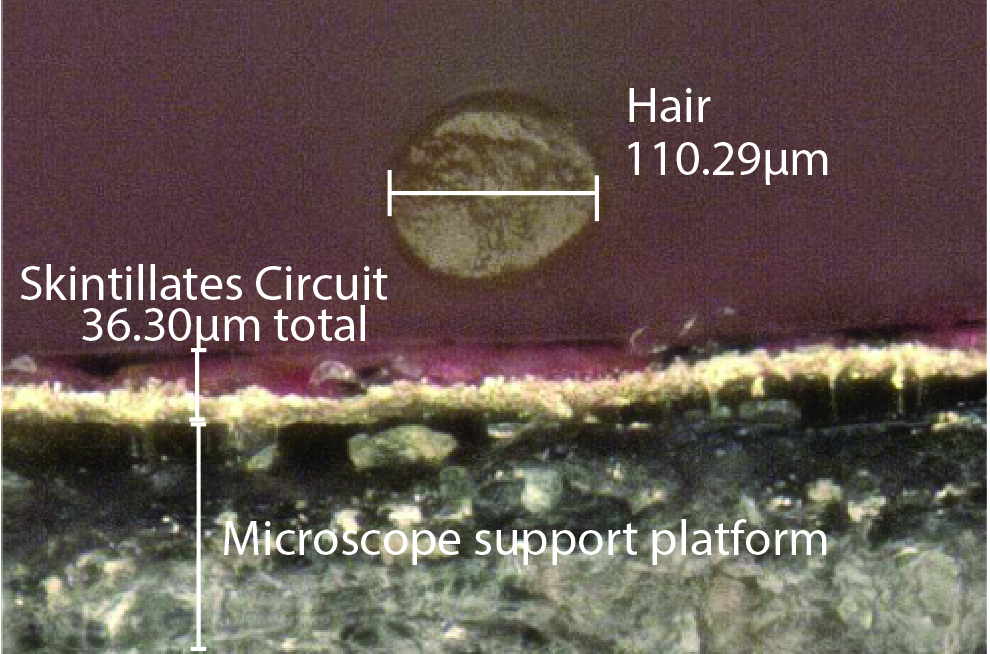
\includegraphics[width=1\columnwidth]{figures/Figure2}
\caption{A micrograph of the cross section of a \SI{36}{\micro\metre}-thick Skintillates device compared to a cross section of a piece of hair (\SI{110}{\micro\metre}).}
\vspace{-8pt}
\label{fig:figure2}
\end{figure}

\subsection{Epidermal Electronics}
Human skin has natural wrinkles, creases, and pits that are on the order of \SI{15}{\micro\metre} to \SI{100}{\micro\metre}. If the wearable electronics have a thickness smaller or comparable to the natural skin features sizes, the wearer will not feel his/her skin unnaturally restrained. The Epidermal Sensor class refers to the class of sensors that are extremely thin, conform to small skin movements such as wrinkling, and present minimal obstructions to users’ skin sensations. Multifunction electronics, such as capacitive sensors that accurately detects physiological signals down to 0.5V, multilayer coils that enable on-skin RF communications, and strain and hydration sensors that aids in post-operation recovery. Materials that are structurally stronger, such as polymeric stamp, water-soluble PVA, or skin-safe stickers are used as a structural backing to transfer the ultra-thin epidermal electronics devices onto the user's skin. Once transferred, the ultra-thin Epidermal electronics (most less than \SI{60}{\micro\metre}), with low Young's modulus that matches with human skin, can be attached to skin through van der Waals force alone. 

Despite these great scientific advances made by the development of epidermal electronics, the fabrication process makes them inaccessible to the general public. The flexibility of epidermal electronics enabled by the ultra-thin geometry that attaches to skin without substrate backing comes at the expense of complicated fabrication method and equipment. The fine gold traces and electrodes (down to \SI{1}{\micro\metre} in width), and the ultra-thin conductive and insulation layers (ranges from 500nm to 5\SI{}{\micro\metre}), though extremely sensitive and conformal to the human skin, requires highly specialized lithographic equipment and etching chemicals to fabricate. In one example application of Epidermal electronics, a small piece of temporary tattoo paper is used as a backing to transfer the epidermal device onto the user's skin. Unfortunately, the etching process that fabricates the fine gold traces is incompatible with commercially available tattoo paper because the paper cannot within the chemicals, thus resulting an additional transfer step. In this study, we aimed to develop a process that can be done without cleanroom equipment, without extreme temperature, but at the same time enable users to customize the device both electronically and aesthetically. 

\section{Fabrication}
\subsection{Material selection}
\begin{enumerate}
  \item The substrate has to be easily customizable to enable artistic expression with the temporary tattoo
  \item The electronic has to be conductive enough to support basic functions. 
  \item The tattoo must be easily applicable, stay on skin for a reasonable amount of time, and removable.
\end{enumerate}
\begin{figure}[!h]
\centering
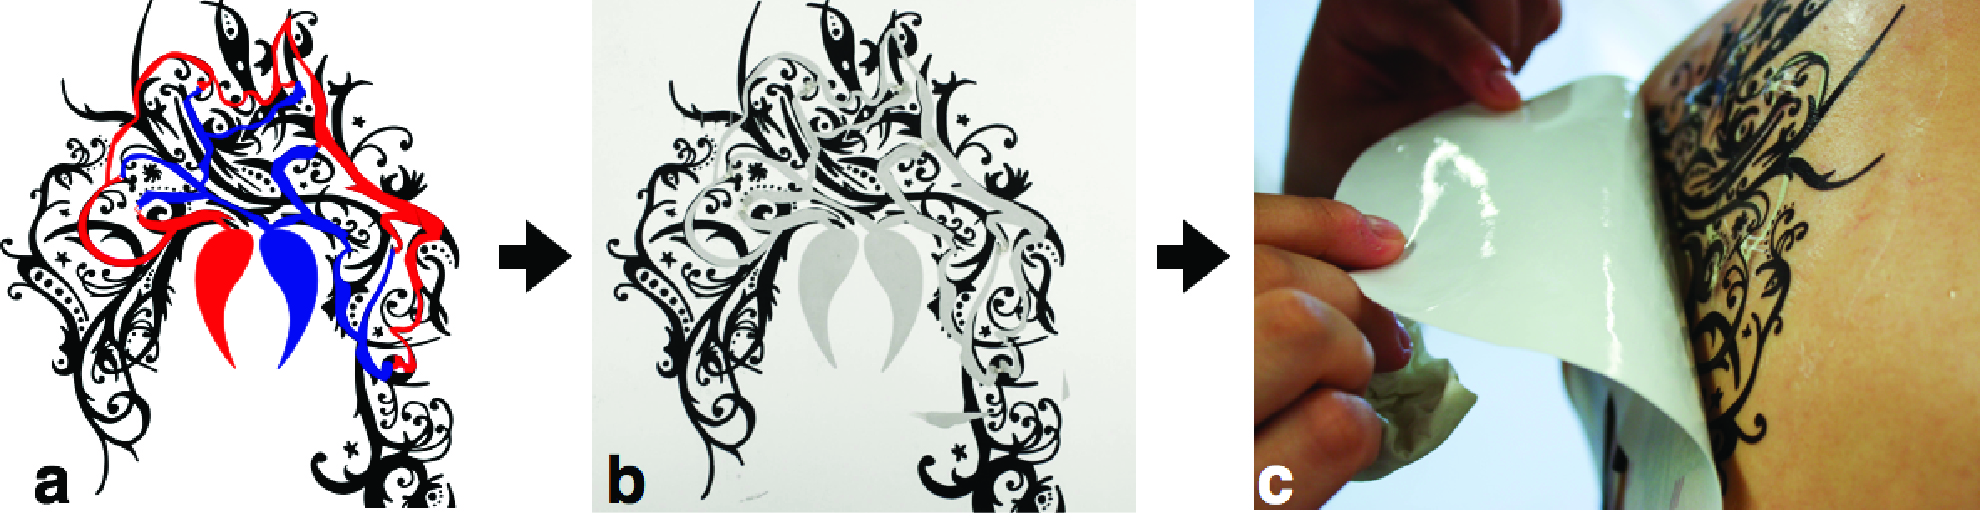
\includegraphics[width=0.9\columnwidth]{figures/Figure3}
\caption{An illustration of the different layers of a basic Skintillate device.}
\label{fig:figure3}
\end{figure}

\begin{figure*}[!b]
\centering
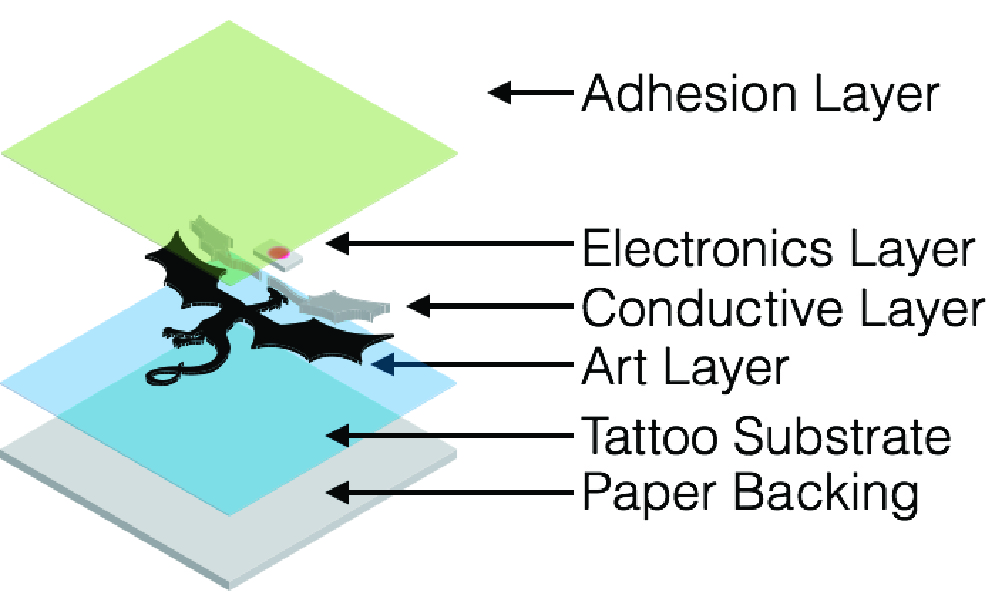
\includegraphics[width=1.0\textwidth]{figures/Figure4}
\caption{With Caption Below, be sure to have a good resolution image
  (see item D within the preparation instructions).}
\label{fig:figure4}
\end{figure*}

Similar to epidermal electronics, we aimed for an integrated-with-skin tattoo aesthetic in Skintiallates. The amplitude of signals that we expect Skintillates to be used with for HCI applications are much larger than the signal strength of what epidermal electronics experiences (down to 500uV). 

With the aforementioned considerations in mind, we chose to directly screenprint the circuits and electronics onto commercially available inkjet printable temporary tattoo papers. The silver ink used in this study was CreativeMaterials 118-38 Screen-printable ink, and the temporary tattoo substrates used is Silhouette Inkjet Printable tattoo paper. Although the Skintillates devices, with conductive ink printed on top of temporary tattoo papers, are not as thin as epidermal electronics, it enables Makers to prototype on-skin interactive wearables with a much more accessible process. (Temporary tattoo papers are commonly used among crafters, it is therefore reasonable to assume that consumers find it acceptable to wear on skin although it’s not as conformable to skin as epidermal electronics.)(reword) Makers can inkjet print their own custom tattoo design, and screenprint the electronics with relatively inexpensive equipment. Screenprinting has also been shown to be able to create extremely fine and complicated electronic structures, and therefore this proposed fabrication method can be adapted by entry level to advanced Makers. 

Due to the need to make a large number of Skintillates display and sensors in this project, we fabricated almost all of the Skintillates devices by screen-printing conductive ink. We have successfully created these devices with conductive inkjet printing and conductive pens, but we will focus on the screen-print method in this paper. 

\subsection{Fabrication Process}

\begin{enumerate}
  \item Design an art layer (nonconductive) with a graphic design tool of choice. Design the circuit and/or sensors to be screen-printed as the conductive layer.
  \item Use an inkjet printer to print the art layer design onto the tattoo substrate (still attached to the paper backing). 
  \item Cut a negative mask with vinyl cutter for screen-printing the conductive layer. 
  \item Apply vinyl mask onto the silkscreen. 
  \item Screen-print the circuit and/or sensors using the silver screen-printing ink.
  \item Let the ink dry in ambient temperature for 3-4 hours or 10 minutes in an oven at 100$^{\circ}$C. 
  \item Mount electronics onto the circuit using z-conductive tape at appropriate locations if needed.   
\end{enumerate}
LED's and resistors of the surface mount 0603 package, which has thickness of  \SI{500}{\micro\metre}, was used throughout this study to minimize increase in thickness in locations where electronics are mounted. Increased complexity in electrical functionality and aesthetic design could be achieved by using deviations of this basic fabrication method. The specific changes will be discussed in the application section. 

\subsection{Designing the Visual Appearance of Skintillates}
explain how covering/or not the conductive layer

\section{Example Applications}
\subsection{On-skin Display}
\begin{figure}[!h]
\centering
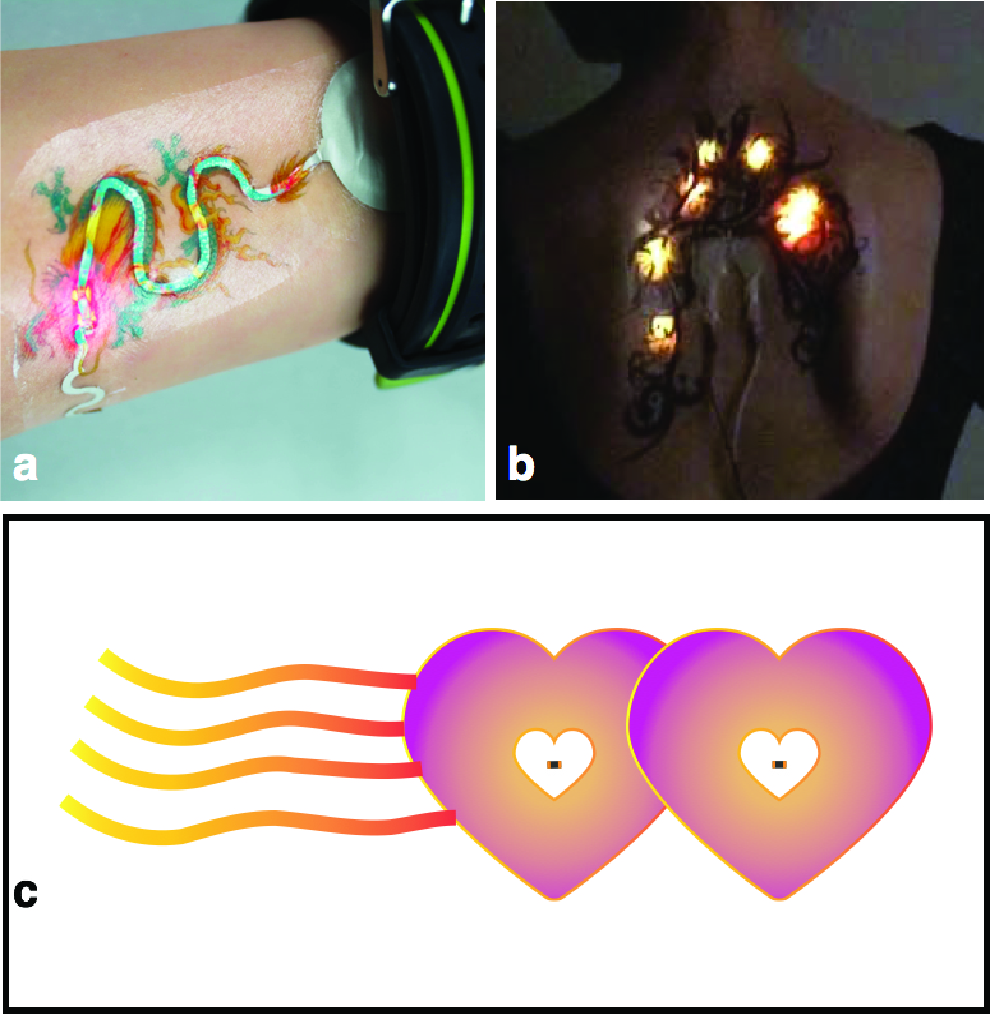
\includegraphics[width=1\columnwidth]{figures/Figure5}
\caption{Example of Skintillates tattoo displays}
\label{fig:figure5}
\end{figure}
One of the most important aspect of wearing tattoos, either temporary or permanent, is to express personal identity. 
Skintillates aims to augment the self-expression of tattoo artwork with electronics. 
In this paper, we present a few examples that we imagine Skintillates to make a useful tattoo display. 
In Figure 5, we show a few examples of decorative Skintilaltes public and private displays. Figure 5a shows a simple dragon tattoo with red LED eyes. The Skintillate dragon tattoo is electrically connected to the watch, and could potentially serve as a point-light display for a smart watch. Figure 5b demonstrates a back tattoo with LED’s that flash with music. The tattoo is controlled by an Arduino hidden under the wearer’s clothing. In this example, we also briefly explored the aesthetic of electronically functionally components on the tattoo. The power pads, which are traditionally circular or square in shape in printed circuit boards, are designed to look like wings to fit with the aesthetic of the art layer of the tattoo. 
In Figure 5c-d, we investigated the potential of using Skintillates as a private wearable display for intimate bio-data. We downloaded two sets of publically available test electrocardiogram (ECG) signals from PhysioNet to simulate the heartbeats from two people. In real-life setting, the Skintillates bio-data display can be interfaced with many of the biomonitoring wearable devices in the market to obtain the data. The LED’s are programmed to blink as the signal strength reaches a certain amplitude (Figure 5c). In Figure 5d, the user wore the Skintillate display under a jacket, which he/she can lift and glance at the private display when desired. 

\subsection{Multi-layer Display}
\begin{figure}[!h]
\centering
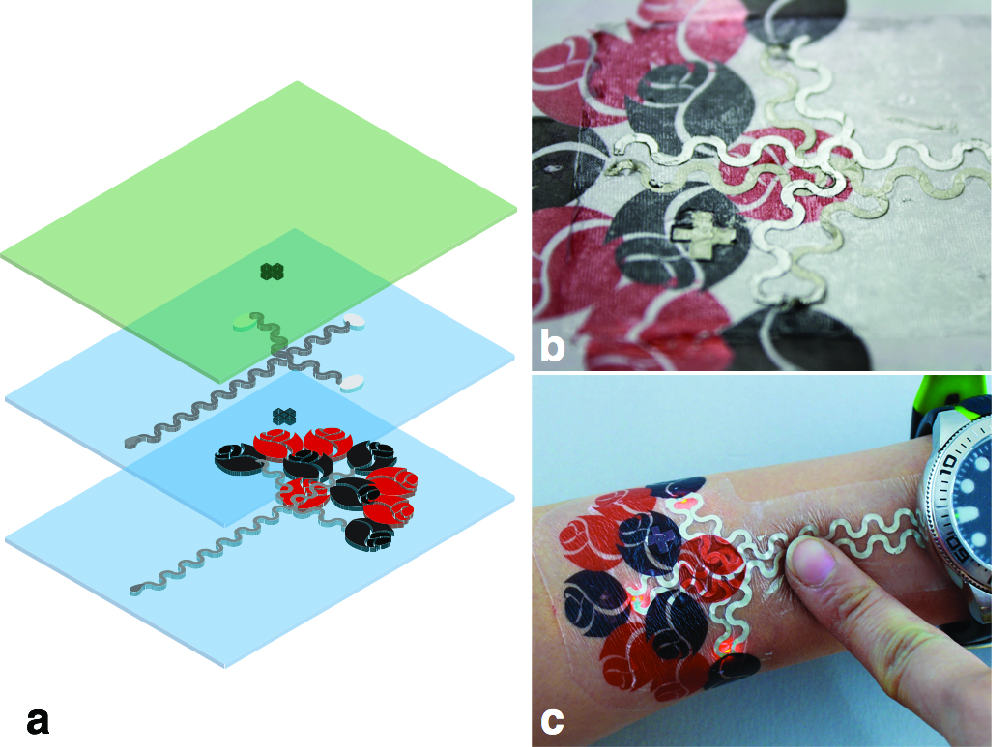
\includegraphics[width=1\columnwidth]{figures/Figure6}
\caption{Multilayer Display}
\label{fig:figure6}
\end{figure}
Multilayer devices can be fabricated for aesthetic or electronic purposes. (Figure 6) In printed circuit board design, multiple layers are often needed to achieve desired form and function. Epidermal electronics have also explored using multilayer device to support more complicated function. In arts practices, layers are often used as a mean to create dimensions (it's an established interactive paradigm for digital design (ask mira) hierarchical design that separate layers and elements). In order to fully explore combining arts and electronics on a wearable device, the Skintillates fabrication should be able to support electronic function and aesthetically attractive multi-layer devices.  

\subsection{Sensing}
\begin{figure*}[!h]
\centering
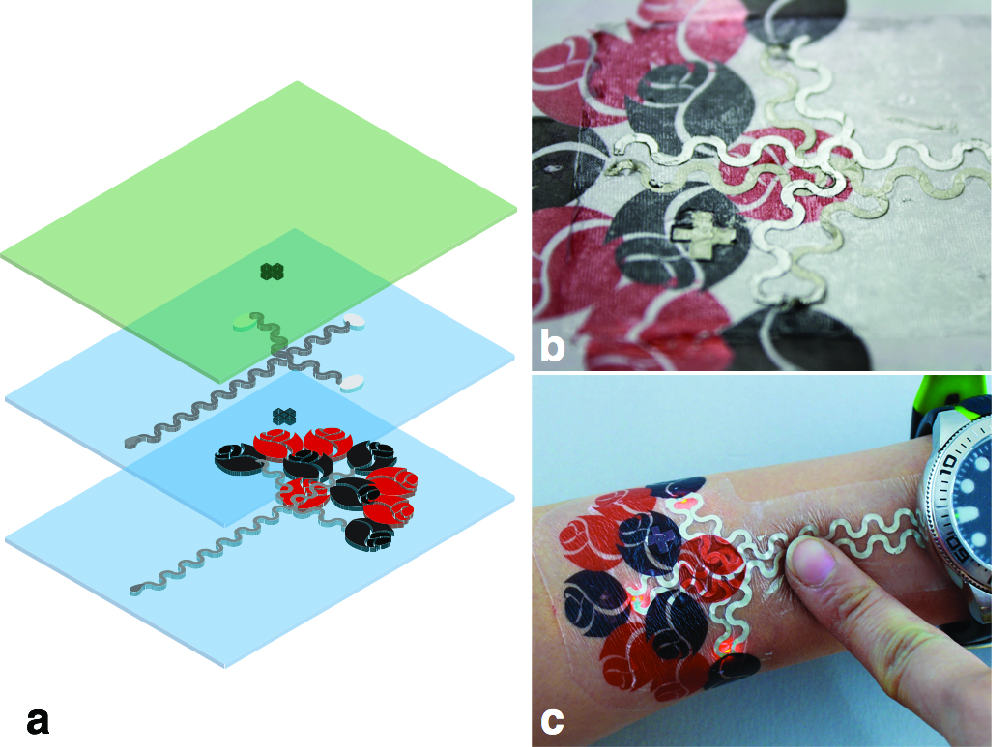
\includegraphics[width=0.8\textwidth]{figures/Figure7}
\caption{Capacitive touch sensing}
\label{fig:figure7}
\end{figure*}
Advanced sensing, including capacitive sensing, using epidermal devices is well-established. In many research studies, various algorithms, data processing methods, and grounding schemes are utilized to overcome any technical difficulties usually associated with wearable sensing. In this paper, we would like to present Skintillates sensors as devices that can be used with interfacing electronics popular amongst makers, the MakeyMakey and the Arduino. Through careful material selections, we can achieve sensitivity suitable for common interactive applications. As mentioned in the Fabrication section, the silver screen printing ink (or most of the silver ink on the market) is very conductive (0.5$\Omega/\square$). The high conductivity is important in resistive switch design, where the touched surface needs to be conductive enough to close the switch; it is also pertinent in capacitor design, where the availability of charge directly affects the sensitivity of the capacitive button (Gauss’s law=$\frac{\sigma}{\epsilon}$). In the following sections, we will go through a few sensing examples using the Skintillates devices. 

\subsection {Capacitive touch}

Capacitive sensing is ubiquitous in interaction design - from sensing gestures to sensing direct touch, the change in electric field carries rich information about the space around us. In this paper, we present Skintillates capacitive buttons that can be used to control mobile devices. To ensure reliable performance of the capacitive sensor, both the electronic filtering and the physical device insulation have be carefully designed. The raw data of the capacitive sensor is shown in Fig xa, from which the signal is then processed and filtered by the Adafruit Capacitive Touch Sensor Breakout MPR121 connected to an Arduino Uno. To insulate the capacitive sensor against the skin where it is attached, we modify the fabrication steps slightly by adding two layers of temporary tattoo substrates on top of the conductive electrodes. (make figures to describe this)
\subsection {On-skin Resistive Sensor}
\begin{figure}[!h]
\centering
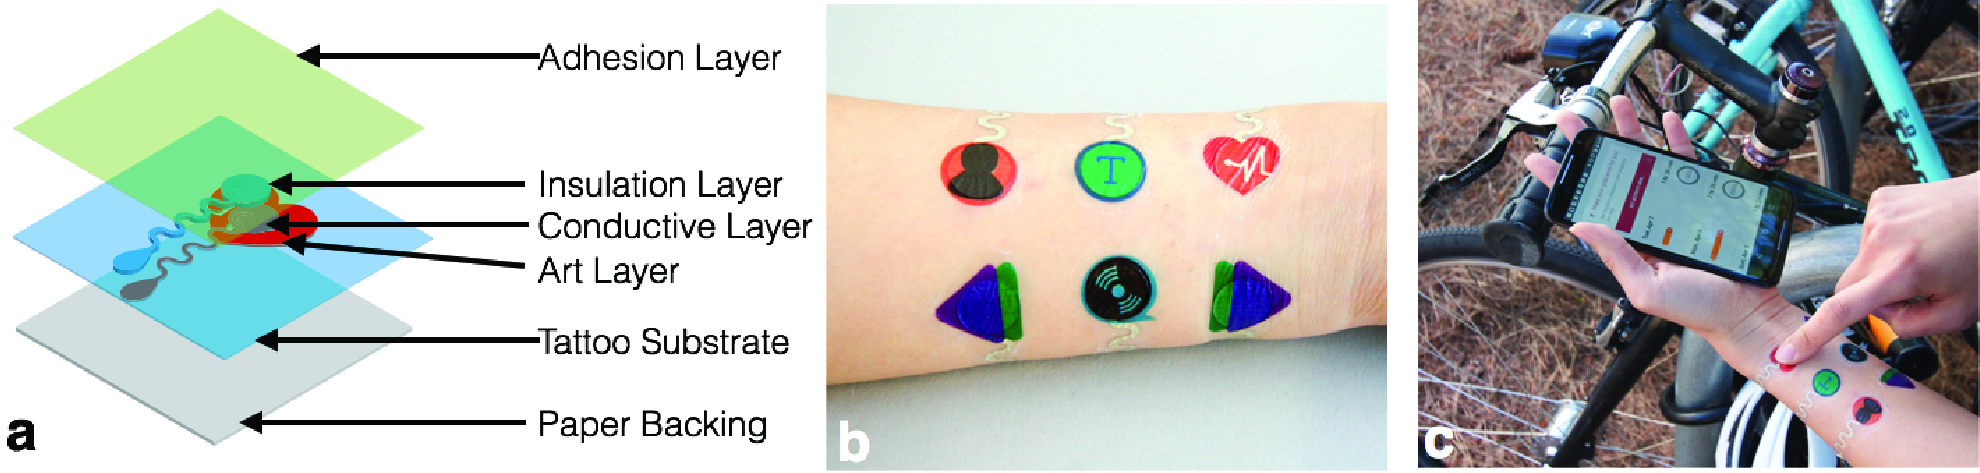
\includegraphics[width=1\columnwidth]{figures/Figure8}
\caption{Example of Skintillates tattoo displays}
\label{fig:figure8}
\end{figure}
Using the human body as a conductor to form a closed circuit to turn on a light is common science experiment, and this sensing method also enable interesting interactions - such as turning bananas into switches - made popular by MakeyMakey. We demonstrated that Skintillates can be used as a resistor sensor that is compatible with MakeyMakey. The construction of the Skintillates resistor sensor is very similar to that of the capacitive sensor - two layers of tattoo substrates are used as an insulative layer beneath the electrode to prevent electrically connection between the sensor and the skin that it is attached to. Figure 8a shows two Skintillates sensors shaped as kites, which are connected to the MakeyMakey to act as the left and right arrow of a computer keyboard. The custom buttons are then used as a controller to play a computer game of moving the kite up and down to avoid hitting objects in the sky. 
\subsection {Strain Gauge}
\begin{figure*}[!h]
\centering
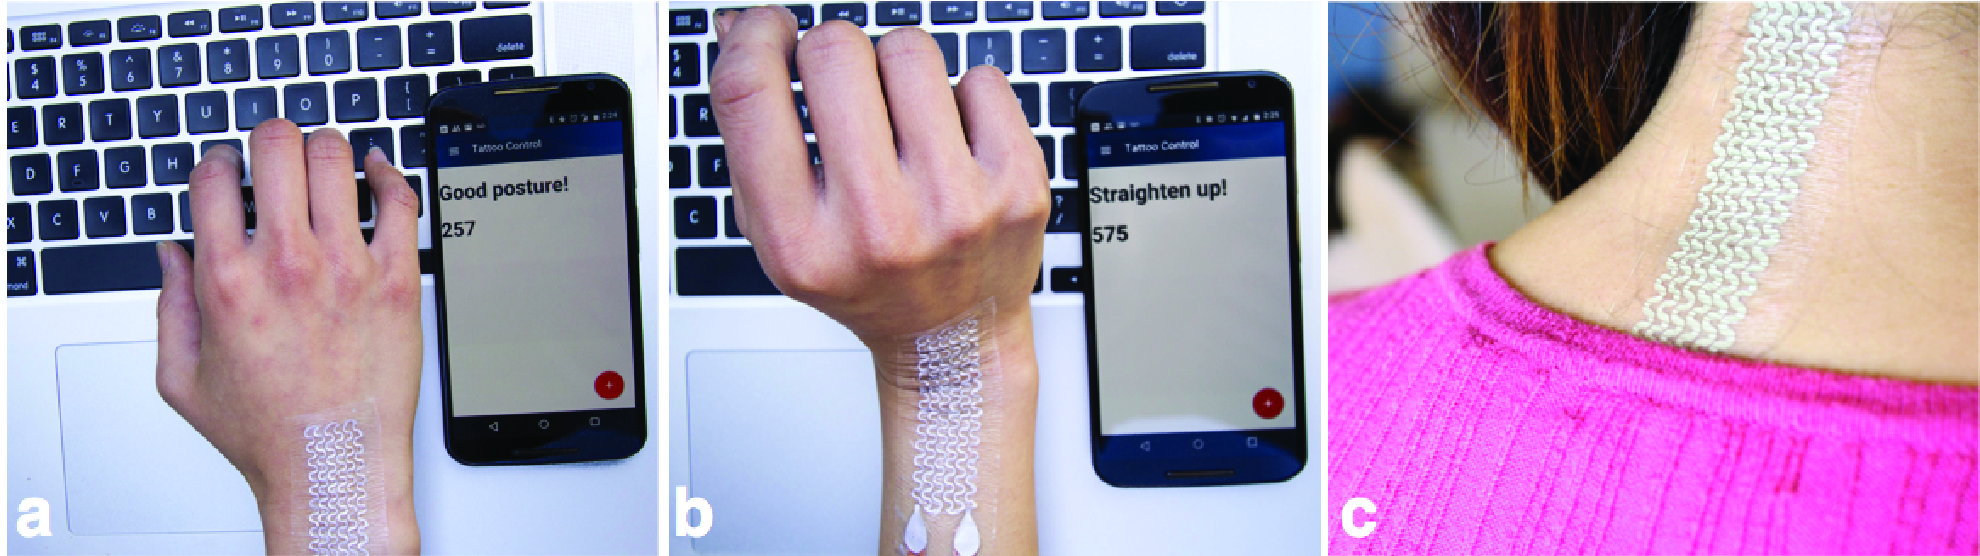
\includegraphics[width=1.0\textwidth]{figures/Figure9}
\caption{Strain gauge for posture sensing}
\label{fig:figure9}
\end{figure*}
The subtle analog motions of the human body carries information that goes beyond the digital on/off button. The Skintillates strain gauge captures the fluid motion of the human body by translating the movement into a variable resistance. The strain gauge has a longer length in the direction of the wrist bending during typing. As the sensor stretches with the wrist, the resistance becomes higher proportionally. The change in resistance is detected through a wheat stone bridge and amplified using the INA125P operational amplifier. Before amplification, the variation in the resistance ranges from 37Ω(when wrist is flat) to 54Ω (The amplified analog value is read using an Arduino Uno and transmitted to a mobile phone via bluetooth. The analog value is displayed on the screen of the mobile phone, and the appropriate warning messages are displayed as the user’s wrist posture change. Although the strain gauge is applied on the wrist in this example, similar application can also be used for back posture by placing the sensor on the neck (Figure 7c). In addition to posture detection, Skintillates strain gauge can be as an alway-available sensor to detect different gestures for electronic interactions or be incorporated into performance art. 

\section {User Study}
In an user study, we asked ten voluntary participants (Fig x, mean age 29.7) to each wear a Skintillates LED display powered with a temporary without any circuit or sensing elements, a 3.3V coin cell battery, and a resistive sensor on a body location of their choice for the duration of a work day, which ranges from 8 to 10 hours. One participant, R7, has a permanent tattoo on upper arm. During which they performed their normal work functions, which mostly includes office activities such as typing, writing, and manipulating light machinery. At the end of the study, participants were asked to rate the wearing comfort of the Skintillates display and imagine the difference personal uses of Skintillates. The Skintillates displays and resistive sensors were all tested at the end of the work day to assess its durability. After the survey, participants were free to remove or keep wearing the Skintillates devices. 

Participants were asked to rate the wearing comfort of the Skintillate display with and without consideration of the battery connection (i.e. copper tape connected to the battery). (have them wear a normal one and rate, this is one more tattoo that i made.) Without considering the battery connection, the wearing comfort of the Skintillates display and resistive sensor have an average rating of 8.21 and 8.76 out of 10 respectively. Most participants describes Skintillates devices as something that they ``don't even feel after a while'' and ``feels very similar to a normal temporary tattoo'', and the 0.5mm-thick 0603 electronic parts as ``little bumps'' and do not significantly affect wearing comfort. When considering the battery connection, the wearing comfort of the display decreased to an average rating of 7.08/10. Participants were most bothered by the dangling battery connections and the hard coin cell battery. One out of ten Skintillate displays was damaged due to a strong tear and separation between the connection wires and the Skintillates device, and all the rest of the nine displays remained perfectly functional at the end of the study.

The majority of the users chose to put the Skintillates devices on their arms, while one user placed the Skintillates display on the back of the neck. (We realize the limitation of this study was that different locations of the skin have different nerve endings and can affect the comfort level. This just shows that this the common locations that we found in this study.) (the elongated shape - potentially less comfortable) When asked about their decision of the placement of the Skintillates devices, users cited the shape of the Skintillates devices and their outfit of the day to be the main drivers. In the follow up survey, user were asked about how long they kept wearing the Skintillates devices. All of the participants (8 out of 10) who have plans to interact with friends and family after the work day kept wearing the tattoo after the study so that they can show the Skintillates devices to their loved ones - ``I wanted to keep it because I thought my kids would think that this is the coolest thing ever''. Two of the participates mentioned that although he/she did not have prior plans to go out after work that night, they decided to go to a public place (one to a restaurant for take-out, and one to a sports bar) to show off the Skintillates display. R7, who went to a sports bar to show off the tattoo, reported ``it seems to be a waste not to show this to someone''. 

All participants reported that they would like to wear the Skintillates device again, as well as express desires to design their own Skintillates displays and sensors. R7 would like to overlay his/her existing permanent tattoo with Skintillate LED displays and sensors. Although all of the participants took off the Skintillates devices before showering or going to bed, all of them said that they took the devices off very carefully as to not damage them. In particular, all of the participants kept the display devices for reuse. 

\ignore{potentially interesting descriptions of the resistive sensor: 
it's like your skin can control things in the house 
can you make a air guitar with sensors on your finger

potentially interesting application of the resistive sensor: 
make a spider man thing
let's put the sensor on your neck - let's put a bone conduction microphone on the back of your neck (omg how engineer is this)

potentially interesting descriptions of the display: 
got nothing for ya. we are all boring nerds that are close to describing the package of the LED's. A lot of us are also married/going out with scientists/engineers. 
potentially interesting application of the display: 
make the display a turn signal for motorcyclists
Burning man! (i'm going to die if i get one more burning man comment)
a pretty baby monitor(from the new dad)
a red/green led to show people whether you want to be bothered at the moment
hook up to sensors to show hydration level (why is everyone freaking out about not drinking enough water??)


(This didn't happen to much because most people went straight home. There were only 4 uninitiated conversation)
In a few of the conversations about the Skintillate devices in which the participants did not initiate, the dangling battery wires were the starting point of conversations. (The other half of initiated by the ``lit-up tattoo'', unsurprisingly.) One participant recounted a conversation happened with a stranger in an elevator, where the stranger initiated the interaction by saying ``are you hooked up to something on your arm''. The dangling wires serves as something that people are somewhat familiar with to strike up a conversation about the novel Skintillates displays.

}






\ignore{Why did you take it home? How long did you keep it on. Who did you show it to. Did you have any public experience. How did you fit this into your daily life? 
Every place: 
Upper arm 
During the course of wearing this, what else would you use it for. Sensing? 
Would you wear this again. Would you wear this on a different location?  

Skintillates was also invited to participate in the two-day exhibition of the National Maker Faire 2015. During which Skintillates LED displays powered by coin cell batteries were given out as part of the exhibit. The LED displays were customized to be a LED lit-up Maker Faire logo, as requested by the event organizer. Users mostly chose to wear the devices on the top of their arms and the outside of their lower legs. The devices were met with great enthusiasm and generated many inspiring conversations. In particular, the displays worn by the event organizer led many Maker Faire participants and potential academic collaborators to visit our booth and offer application suggestions such as displays for events like Burning Man, medical electrodes for children, or custom motion controller for robots.} 


\section {Limitations}
Although Skintillates provides tremendous new features and benefits to creating novel wearable electronics, there are several limitations. First, although the Skintillates device is highly flexible, the electrical connection, currently made with copper tape, is not. In additional to creating discomfort, the difference in material  properties causes the electrical connection to be the mechanically weakest point of the device. This problem can be overcome by stabilizing the connection using a small piece of medical-grade tape - the tape relieve most of the stress exert on the connection and prevent tearing of the connection. In future work, we would like to develop a flexible electrical connector that can move with the skin and provide an electrical interface with the Skintillate device. 

Another limitation lies in the reusability of the Skintillates devices. In the research team's experience, the Skintilltaes devices can be reused at least four to five times if the devices contains finely traced (<2mm) circuits and many more times if the for sensors with large conductive patches. The reusability of the devices could potentially be improved with a thin (<10um) spray-on encapsulating layer. Further studies can also be performed to optimize the electronic design for durability. 

\section {Discussion and future applications}

\section {conclusion}
 \cite{Kim:2015ii}.



\section{Acknowledgments}

We thank CHI, PDC and CSCW volunteers, and all publications support
and staff, who wrote and provided helpful comments on previous
versions of this document.  Some of the references cited in this paper
are included for illustrative purposes only.  \textbf{Don't forget
to acknowledge funding sources as well}, so you don't wind up
having to correct it later.

% Balancing columns in a ref list is a bit of a pain because you
% either use a hack like flushend or balance, or manually insert
% a column break.  http://www.tex.ac.uk/cgi-bin/texfaq2html?label=balance
% multicols doesn't work because we're already in two-column mode,
% and flushend isn't awesome, so I choose balance.  See this
% for more info: http://cs.brown.edu/system/software/latex/doc/balance.pdf
%
% Note that in a perfect world balance wants to be in the first
% column of the last page.
%
% If balance doesn't work for you, you can remove that and
% hard-code a column break into the bbl file right before you
% submit:
%
% http://stackoverflow.com/questions/2149854/how-to-manually-equalize-columns-
% in-an-ieee-paper-if-using-bibtex
%
% Or, just remove \balance and give up on balancing the last page.
%
\balance

\bibliographystyle{acm-sigchi}
\bibliography{skintillates}
\end{document}
